\chapter{Requirement Analysis}
\label{chap:requirement-analysis}

\section{Stakeholder Analysis}
\label{section:stakeholder-analysis}
\begin{enumerate}
    \item \textbf{People who are exposed to danger more than others} \\
    This group includes individuals whose lifestyle, occupation, health conditions, or environmental factors place them at elevated risk for emergencies. These stakeholders have a higher statistical likelihood of experiencing emergencies and often face them in challenging contexts. They need a solution that addresses their specific risk factors and can provide tailored guidance for their particular situations. ByStander's AI-powered contextual awareness and specialized guidance for different emergency types directly addresses their elevated risk profile.

    \item \textbf{Caregivers of a patient or family members} \\
    Those responsible for vulnerable individuals, such as the elderly, people with medical conditions, or children who cannot assist themselves. Caregivers often face high-stress emergency situations involving individuals with complex medical needs. They need specialized guidance that accounts for the specific conditions of those in their care. ByStander provides condition-specific emergency protocols and can store critical medical information for quick retrieval during emergencies, allowing caregivers to respond more effectively while managing their own stress

    \item \textbf{Emergency Sevice Operator} \\
    Police, hospitals, and first responders who receive emergency calls. Emergency operators face significant challenges in quickly gathering accurate information from callers who are often in panic states and unable to communicate effectively. ByStander's ability to compile structured emergency reports with precise location data, automatically gather key medical information, and facilitate clearer communication directly addresses their operational challenges. The app becomes a valuable intermediary that improves information quality and reduces time-to-dispatch.

    \item \textbf{Medical Professionals or Emergency Officers (Indirect Stakeholders)} \\
    Healthcare providers, paramedics, and first-aid trainers who contribute to emergency guidance. Though not direct users of the app, these professionals benefit significantly from the improved emergency response it facilitates. Some of them arrive at scenes where better initial actions have been taken, receive more complete information about the emergency, and encounter patients who have received appropriate preliminary care. This improves their ability to provide effective treatment and potentially leads to better outcomes.
\end{enumerate}

\section{User Stories}
\label{section:user-stories}
\begin{enumerate}
    \item \textbf{People who are exposed to danger more than others}
    \begin{itemize}
        \item As someone working in a high-risk environment, I want quick access to emergency procedures so I can provide proper care until professional help arrives.
        \item As a person who frequently works alone, I need to easily identify which emergency service to contact first so I can ensure the fastest response in critical situations.
        \item As someone who visits unfamiliar locations regularly, I want location-aware emergency facility recommendations so I can contact the closest appropriate help regardless of where I am.
        \item As a worker in a hazardous industrial setting, I need pre-written emergency scripts for different types of accidents so I can provide precise details about chemical exposure or machinery injuries when under extreme stress.
    \end{itemize}

    \item \textbf{Caregivers of a patient or family members}
    \begin{itemize}
        \item As someone responsible for a patient with mobility issues, I need location-based facility recommendations that consider accessibility so I can choose appropriate emergency services.
        \item As a caregiver who may need to make quick decisions, I want clear step-by-step guidance for common emergency situations related to my patient's condition so I can act confidently during a crisis.
        \item As someone caring for a non-verbal child with special needs, I want emergency scripts that include their specific diagnosis, behaviors, and needs so medical professionals can provide appropriate care immediately.
    \end{itemize}
    
    \item \textbf{Emergency Operator}
    \begin{itemize}
        \item As an emergency operator handling diverse calls, I want callers to provide clear, structured information so I can quickly assess the situation and dispatch appropriate resources.
        \item As someone coordinating emergency responses, I need callers to accurately communicate their location and the nature of the emergency so I can send the right help to the right place.
        \item As an emergency responder coordinator, I need callers to understand which details are most important to share first so I can prioritize response appropriately.
        \item As an operator handling calls from unfamiliar areas, I want callers to be aware of nearby emergency facilities so I can coordinate with the most appropriate local resources.
    \end{itemize}

    \item \textbf{Medical Professionals or Emergency Officers (Indirect Stakeholders)}
    \begin{itemize}
        \item As an emergency responder arriving at a scene, I need civilians to have taken appropriate initial actions so the situation hasn't worsened during wait time.
        \item As a hospital emergency staff member, I want incoming patients to be directed to the most appropriate facility for their condition so resources are used efficiently across the healthcare system.
        \item As a medical professional dealing with time-sensitive emergencies, I want patients to arrive at facilities that can immediately address their specific needs so treatment isn't delayed by subsequent transfers.

    \end{itemize}

\end{enumerate}

\section{Use Case Diagram}
\label{section:use-case-diagram}
<TIP: Write a use case diagram for your project here. Refer to an
article “What is a use case diagram?” by Lucidchart for help./>

\section{Use Case Model}
\label{section:use-case-model}
A use case is a detailed description of how a system
interacts with an external entity (such as a user or another system) to
accomplish a specific goal. Use cases provide a high-level view of the
functionality of a system and help in capturing and documenting its
requirements from the perspective of end users.

<TIP: Write use cases for your project here. Make sure to use the
appropriate type of use case for each scenario (brief, casual, and fully-dressed
use case)./>

\section{User Interface Design}
\label{section:user-interface-design}
This is the tentative UI design of ByStander

\begin{figure}[h]
    \centering
    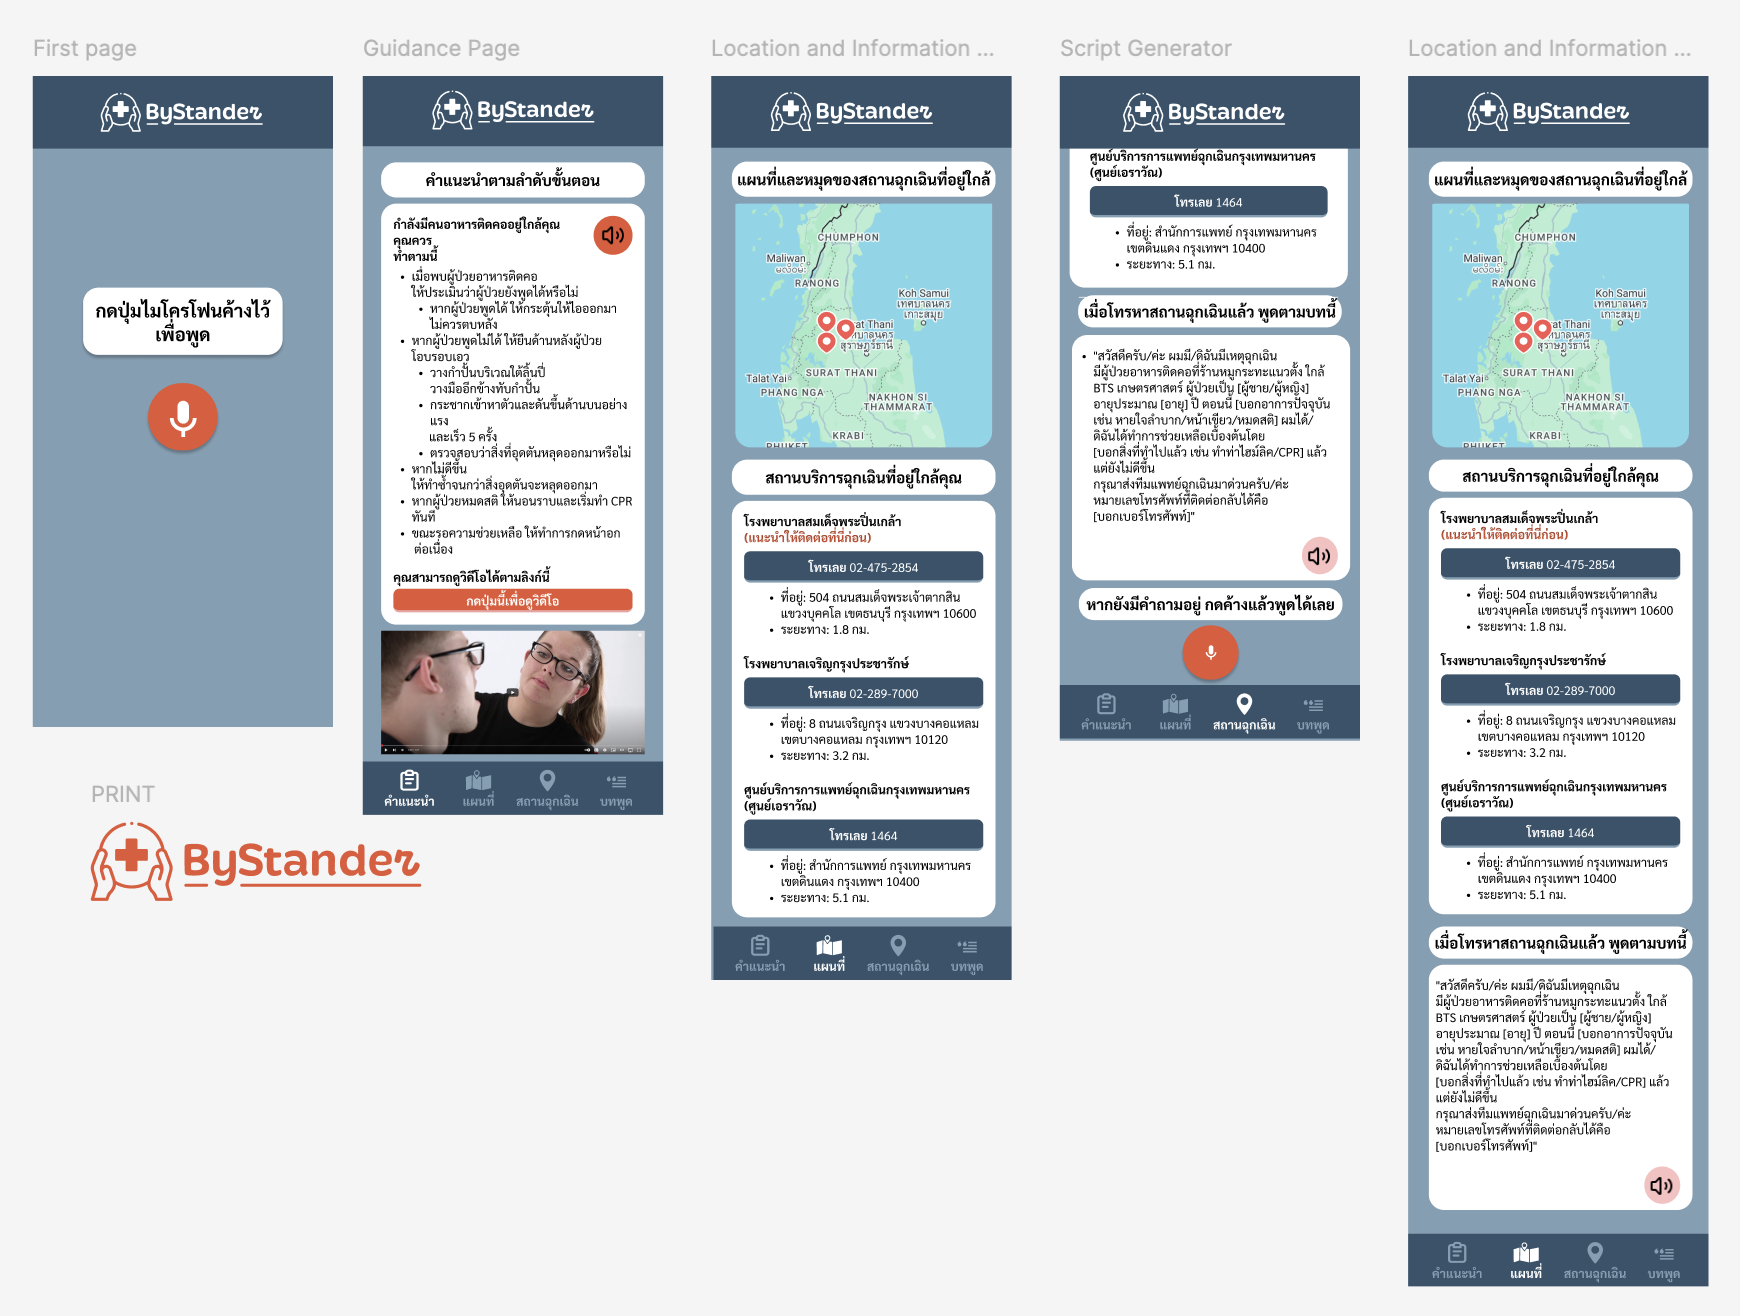
\includegraphics[width=0.9\textwidth]{/design/initial-ui-design.png}
    \caption{User Interface Design}
\end{figure}